\section{Experimental Results}\label{sec:experiment}
\subsection{Experimental Setup}

CPU:Intel(R) Xeon(R) Gold 5218R CPU @ 2.10GHz,Memory:64G,8Thread;FPGA, xcvu9p,8 computing cores in parallel


\subsection{Maze Routing Acceleration}

% Please add the following required packages to your document preamble:
% \usepackage{multirow}
% \begin{table*}[!htbp]
%     \caption{Comparison of performance between TritonRoute [?] Dr.CU and our FPGA acceleration to complete batched maze routing kernel with ISPD 2018 [?] contest benchmarks.}
%     \begin{tabular}{|c|ccll|clll|llll|lllc|cccl|cl|}
%     \hline
%     \multirow{2}{*}{Benchmark} & \multicolumn{4}{c|}{Wirelength(um)}                                                                             & \multicolumn{4}{c|}{Via count}                                                                                  & \multicolumn{4}{c|}{Memory(GB)}                                                                                 & \multicolumn{4}{c|}{\begin{tabular}[c]{@{}c@{}}ISPD' 18 \\ quality score\end{tabular}}     & \multicolumn{4}{c|}{\begin{tabular}[c]{@{}c@{}}Routing Kernel\\ Runtime(s)\end{tabular}}                            & \multicolumn{2}{c|}{\begin{tabular}[c]{@{}c@{}}Routing Kernel\\ Speed-up\end{tabular}} \\ \cline{2-23} 
%                                & \multicolumn{1}{c|}{TR} & \multicolumn{1}{c|}{CU} & \multicolumn{1}{c|}{MAcc-TR} & \multicolumn{1}{c|}{MAcc-CU} & \multicolumn{1}{c|}{TR} & \multicolumn{1}{c|}{CU} & \multicolumn{1}{c|}{MAcc-TR} & \multicolumn{1}{c|}{MAcc-CU} & \multicolumn{1}{c|}{TR} & \multicolumn{1}{c|}{CU} & \multicolumn{1}{c|}{MAcc-TR} & \multicolumn{1}{c|}{MAcc-CU} & \multicolumn{1}{c|}{TR} & \multicolumn{1}{c|}{CU} & \multicolumn{1}{c|}{MAcc-TR} & MAcc-CU & \multicolumn{1}{c|}{TR}     & \multicolumn{1}{c|}{CU} & \multicolumn{1}{c|}{MAcc-TR} & \multicolumn{1}{c|}{MAcc-CU} & \multicolumn{1}{c|}{MAcc-TR}               & \multicolumn{1}{c|}{MAcc-CU}              \\ \hline
%     ispd18\_testl              & \multicolumn{1}{c|}{}   & \multicolumn{1}{c|}{}   & \multicolumn{1}{l|}{}        &                              & \multicolumn{1}{c|}{}   & \multicolumn{1}{l|}{}   & \multicolumn{1}{l|}{}        &                              & \multicolumn{1}{l|}{}   & \multicolumn{1}{l|}{}   & \multicolumn{1}{l|}{}        &                              & \multicolumn{1}{l|}{}   & \multicolumn{1}{l|}{}   & \multicolumn{1}{l|}{}        &         & \multicolumn{1}{c|}{4.41}   & \multicolumn{1}{c|}{}   & \multicolumn{1}{c|}{2.03}    &                              & \multicolumn{1}{c|}{2.2x}                  &                                           \\ \hline
%     ispd18\_test2              & \multicolumn{1}{c|}{}   & \multicolumn{1}{c|}{}   & \multicolumn{1}{l|}{}        &                              & \multicolumn{1}{c|}{}   & \multicolumn{1}{l|}{}   & \multicolumn{1}{l|}{}        &                              & \multicolumn{1}{l|}{}   & \multicolumn{1}{l|}{}   & \multicolumn{1}{l|}{}        &                              & \multicolumn{1}{l|}{}   & \multicolumn{1}{l|}{}   & \multicolumn{1}{l|}{}        &         & \multicolumn{1}{c|}{58.86}  & \multicolumn{1}{c|}{}   & \multicolumn{1}{c|}{25.93}   &                              & \multicolumn{1}{c|}{2.3x}                  &                                           \\ \hline
%     ispd18\_test3              & \multicolumn{1}{c|}{}   & \multicolumn{1}{c|}{}   & \multicolumn{1}{l|}{}        &                              & \multicolumn{1}{c|}{}   & \multicolumn{1}{l|}{}   & \multicolumn{1}{l|}{}        &                              & \multicolumn{1}{l|}{}   & \multicolumn{1}{l|}{}   & \multicolumn{1}{l|}{}        &                              & \multicolumn{1}{l|}{}   & \multicolumn{1}{l|}{}   & \multicolumn{1}{l|}{}        &         & \multicolumn{1}{c|}{110.07} & \multicolumn{1}{c|}{}   & \multicolumn{1}{c|}{52.4}    &                              & \multicolumn{1}{c|}{2.1x}                  &                                           \\ \hline
%     ispd18\_test4              & \multicolumn{1}{c|}{}   & \multicolumn{1}{c|}{}   & \multicolumn{1}{l|}{}        &                              & \multicolumn{1}{c|}{}   & \multicolumn{1}{l|}{}   & \multicolumn{1}{l|}{}        &                              & \multicolumn{1}{l|}{}   & \multicolumn{1}{l|}{}   & \multicolumn{1}{l|}{}        &                              & \multicolumn{1}{l|}{}   & \multicolumn{1}{l|}{}   & \multicolumn{1}{l|}{}        &         & \multicolumn{1}{c|}{244.48} & \multicolumn{1}{c|}{}   & \multicolumn{1}{c|}{211.68}  &                              & \multicolumn{1}{c|}{2.3x}                  &                                           \\ \hline
%     ispd18\_test5              & \multicolumn{1}{c|}{}   & \multicolumn{1}{c|}{}   & \multicolumn{1}{l|}{}        &                              & \multicolumn{1}{c|}{}   & \multicolumn{1}{l|}{}   & \multicolumn{1}{l|}{}        &                              & \multicolumn{1}{l|}{}   & \multicolumn{1}{l|}{}   & \multicolumn{1}{l|}{}        &                              & \multicolumn{1}{l|}{}   & \multicolumn{1}{l|}{}   & \multicolumn{1}{l|}{}        &         & \multicolumn{1}{c|}{109.42} & \multicolumn{1}{c|}{}   & \multicolumn{1}{c|}{40.39}   &                              & \multicolumn{1}{c|}{2.3x}                  &                                           \\ \hline
%     ispd18\_test6              & \multicolumn{1}{c|}{}   & \multicolumn{1}{c|}{}   & \multicolumn{1}{l|}{}        &                              & \multicolumn{1}{c|}{}   & \multicolumn{1}{l|}{}   & \multicolumn{1}{l|}{}        &                              & \multicolumn{1}{l|}{}   & \multicolumn{1}{l|}{}   & \multicolumn{1}{l|}{}        &                              & \multicolumn{1}{l|}{}   & \multicolumn{1}{l|}{}   & \multicolumn{1}{l|}{}        &         & \multicolumn{1}{c|}{165.39} & \multicolumn{1}{c|}{}   & \multicolumn{1}{c|}{77.33}   &                              & \multicolumn{1}{c|}{2.1x}                  &                                           \\ \hline
%     ispd18\_test7              & \multicolumn{1}{c|}{}   & \multicolumn{1}{c|}{}   & \multicolumn{1}{l|}{}        &                              & \multicolumn{1}{c|}{}   & \multicolumn{1}{l|}{}   & \multicolumn{1}{l|}{}        &                              & \multicolumn{1}{l|}{}   & \multicolumn{1}{l|}{}   & \multicolumn{1}{l|}{}        &                              & \multicolumn{1}{l|}{}   & \multicolumn{1}{l|}{}   & \multicolumn{1}{l|}{}        &         & \multicolumn{1}{c|}{246.12} & \multicolumn{1}{c|}{}   & \multicolumn{1}{c|}{111.98}  &                              & \multicolumn{1}{c|}{2.2x}                  &                                           \\ \hline
%     ispd18\_test8              & \multicolumn{1}{c|}{}   & \multicolumn{1}{c|}{}   & \multicolumn{1}{l|}{}        &                              & \multicolumn{1}{c|}{}   & \multicolumn{1}{l|}{}   & \multicolumn{1}{l|}{}        &                              & \multicolumn{1}{l|}{}   & \multicolumn{1}{l|}{}   & \multicolumn{1}{l|}{}        &                              & \multicolumn{1}{l|}{}   & \multicolumn{1}{l|}{}   & \multicolumn{1}{l|}{}        &         & \multicolumn{1}{c|}{256.73} & \multicolumn{1}{c|}{}   & \multicolumn{1}{c|}{125.29}  &                              & \multicolumn{1}{c|}{2.1x}                  &                                           \\ \hline
%     ispd18\_test9              & \multicolumn{1}{c|}{}   & \multicolumn{1}{c|}{}   & \multicolumn{1}{l|}{}        &                              & \multicolumn{1}{c|}{}   & \multicolumn{1}{l|}{}   & \multicolumn{1}{l|}{}        &                              & \multicolumn{1}{l|}{}   & \multicolumn{1}{l|}{}   & \multicolumn{1}{l|}{}        &                              & \multicolumn{1}{l|}{}   & \multicolumn{1}{l|}{}   & \multicolumn{1}{l|}{}        &         & \multicolumn{1}{c|}{264.21} & \multicolumn{1}{c|}{}   & \multicolumn{1}{c|}{128.19}  &                              & \multicolumn{1}{c|}{2.1x}                  &                                           \\ \hline
%     ispd18\_test10             & \multicolumn{1}{c|}{}   & \multicolumn{1}{c|}{}   & \multicolumn{1}{l|}{}        &                              & \multicolumn{1}{c|}{}   & \multicolumn{1}{l|}{}   & \multicolumn{1}{l|}{}        &                              & \multicolumn{1}{l|}{}   & \multicolumn{1}{l|}{}   & \multicolumn{1}{l|}{}        &                              & \multicolumn{1}{l|}{}   & \multicolumn{1}{l|}{}   & \multicolumn{1}{l|}{}        &         & \multicolumn{1}{c|}{380.69} & \multicolumn{1}{c|}{}   & \multicolumn{1}{c|}{180.455} &                              & \multicolumn{1}{c|}{2.1x}                  &                                           \\ \hline
%     \end{tabular}
%     \label{tab:wide_table}
%     \end{table*}
% Please add the following required packages to your document preamble:
% \usepackage{multirow}
% Please add the following required packages to your document preamble:
% \usepackage{multirow}
% \begin{table*}[!htbp]
%     \centering
%     \caption{Comparison of performance between TritonRoute [?] Dr.CU and our FPGA acceleration to complete batched maze routing kernel with ISPD 2018 [?] contest benchmarks.}
%     \begin{tabularx}{\textwidth}{|c|ccll|clll|lllc|cccl|cl|}
%     \hline
%     \multirow{2}{*}{ispd18} & \multicolumn{4}{c|}{Wirelength(um)}                                                                                                                                                                   & \multicolumn{4}{c|}{Via count}                                                                                                                                                                        & \multicolumn{4}{c|}{\begin{tabular}[c]{@{}c@{}}ISPD' 18 \\ quality score\end{tabular}}                                                                                           & \multicolumn{4}{c|}{\begin{tabular}[c]{@{}c@{}}Routing Kernel\\ Runtime(s)\end{tabular}}                                                                                                                  & \multicolumn{2}{c|}{\begin{tabular}[c]{@{}c@{}}Routing Kernel\\ Speed-up\end{tabular}}                                                            \\ \cline{2-19} 
%                             & \multicolumn{1}{c|}{TR} & \multicolumn{1}{c|}{CU} & \multicolumn{1}{c|}{\begin{tabular}[c]{@{}c@{}}MAcc\\ -TR\end{tabular}} & \multicolumn{1}{c|}{\begin{tabular}[c]{@{}c@{}}MAcc\\ -CU\end{tabular}} & \multicolumn{1}{c|}{TR} & \multicolumn{1}{c|}{CU} & \multicolumn{1}{c|}{\begin{tabular}[c]{@{}c@{}}MAcc\\ -TR\end{tabular}} & \multicolumn{1}{c|}{\begin{tabular}[c]{@{}c@{}}MAcc\\ -CU\end{tabular}} & \multicolumn{1}{c|}{TR} & \multicolumn{1}{c|}{CU} & \multicolumn{1}{c|}{\begin{tabular}[c]{@{}c@{}}MAcc\\ -TR\end{tabular}} & \begin{tabular}[c]{@{}c@{}}MAcc\\ -CU\end{tabular} & \multicolumn{1}{c|}{TR}     & \multicolumn{1}{c|}{CU} & \multicolumn{1}{c|}{\begin{tabular}[c]{@{}c@{}}MAcc\\ -TR\end{tabular}} & \multicolumn{1}{c|}{\begin{tabular}[c]{@{}c@{}}MAcc\\ -CU\end{tabular}} & \multicolumn{1}{c|}{\begin{tabular}[c]{@{}c@{}}MAcc\\ -TR\end{tabular}} & \multicolumn{1}{c|}{\begin{tabular}[c]{@{}c@{}}MAcc\\ -CU\end{tabular}} \\ \hline
%     testl                   & \multicolumn{1}{c|}{}   & \multicolumn{1}{c|}{}   & \multicolumn{1}{l|}{}                                                   &                                                                         & \multicolumn{1}{c|}{}   & \multicolumn{1}{l|}{}   & \multicolumn{1}{l|}{}                                                   &                                                                         & \multicolumn{1}{l|}{}   & \multicolumn{1}{l|}{}   & \multicolumn{1}{l|}{}                                                   &                                                    & \multicolumn{1}{c|}{4.41}   & \multicolumn{1}{c|}{}   & \multicolumn{1}{c|}{2.03}                                               &                                                                         & \multicolumn{1}{c|}{2.2x}                                               &                                                                         \\ \hline
%     test2                   & \multicolumn{1}{c|}{}   & \multicolumn{1}{c|}{}   & \multicolumn{1}{l|}{}                                                   &                                                                         & \multicolumn{1}{c|}{}   & \multicolumn{1}{l|}{}   & \multicolumn{1}{l|}{}                                                   &                                                                         & \multicolumn{1}{l|}{}   & \multicolumn{1}{l|}{}   & \multicolumn{1}{l|}{}                                                   &                                                    & \multicolumn{1}{c|}{58.86}  & \multicolumn{1}{c|}{}   & \multicolumn{1}{c|}{25.93}                                              &                                                                         & \multicolumn{1}{c|}{2.3x}                                               &                                                                         \\ \hline
%     test3                   & \multicolumn{1}{c|}{}   & \multicolumn{1}{c|}{}   & \multicolumn{1}{l|}{}                                                   &                                                                         & \multicolumn{1}{c|}{}   & \multicolumn{1}{l|}{}   & \multicolumn{1}{l|}{}                                                   &                                                                         & \multicolumn{1}{l|}{}   & \multicolumn{1}{l|}{}   & \multicolumn{1}{l|}{}                                                   &                                                    & \multicolumn{1}{c|}{110.07} & \multicolumn{1}{c|}{}   & \multicolumn{1}{c|}{52.4}                                               &                                                                         & \multicolumn{1}{c|}{2.1x}                                               &                                                                         \\ \hline
%     test4                   & \multicolumn{1}{c|}{}   & \multicolumn{1}{c|}{}   & \multicolumn{1}{l|}{}                                                   &                                                                         & \multicolumn{1}{c|}{}   & \multicolumn{1}{l|}{}   & \multicolumn{1}{l|}{}                                                   &                                                                         & \multicolumn{1}{l|}{}   & \multicolumn{1}{l|}{}   & \multicolumn{1}{l|}{}                                                   &                                                    & \multicolumn{1}{c|}{244.48} & \multicolumn{1}{c|}{}   & \multicolumn{1}{c|}{211.68}                                             &                                                                         & \multicolumn{1}{c|}{2.3x}                                               &                                                                         \\ \hline
%     test5                   & \multicolumn{1}{c|}{}   & \multicolumn{1}{c|}{}   & \multicolumn{1}{l|}{}                                                   &                                                                         & \multicolumn{1}{c|}{}   & \multicolumn{1}{l|}{}   & \multicolumn{1}{l|}{}                                                   &                                                                         & \multicolumn{1}{l|}{}   & \multicolumn{1}{l|}{}   & \multicolumn{1}{l|}{}                                                   &                                                    & \multicolumn{1}{c|}{109.42} & \multicolumn{1}{c|}{}   & \multicolumn{1}{c|}{40.39}                                              &                                                                         & \multicolumn{1}{c|}{2.3x}                                               &                                                                         \\ \hline
%     test6                   & \multicolumn{1}{c|}{}   & \multicolumn{1}{c|}{}   & \multicolumn{1}{l|}{}                                                   &                                                                         & \multicolumn{1}{c|}{}   & \multicolumn{1}{l|}{}   & \multicolumn{1}{l|}{}                                                   &                                                                         & \multicolumn{1}{l|}{}   & \multicolumn{1}{l|}{}   & \multicolumn{1}{l|}{}                                                   &                                                    & \multicolumn{1}{c|}{165.39} & \multicolumn{1}{c|}{}   & \multicolumn{1}{c|}{77.33}                                              &                                                                         & \multicolumn{1}{c|}{2.1x}                                               &                                                                         \\ \hline
%     test7                   & \multicolumn{1}{c|}{}   & \multicolumn{1}{c|}{}   & \multicolumn{1}{l|}{}                                                   &                                                                         & \multicolumn{1}{c|}{}   & \multicolumn{1}{l|}{}   & \multicolumn{1}{l|}{}                                                   &                                                                         & \multicolumn{1}{l|}{}   & \multicolumn{1}{l|}{}   & \multicolumn{1}{l|}{}                                                   &                                                    & \multicolumn{1}{c|}{246.12} & \multicolumn{1}{c|}{}   & \multicolumn{1}{c|}{111.98}                                             &                                                                         & \multicolumn{1}{c|}{2.2x}                                               &                                                                         \\ \hline
%     test8                   & \multicolumn{1}{c|}{}   & \multicolumn{1}{c|}{}   & \multicolumn{1}{l|}{}                                                   &                                                                         & \multicolumn{1}{c|}{}   & \multicolumn{1}{l|}{}   & \multicolumn{1}{l|}{}                                                   &                                                                         & \multicolumn{1}{l|}{}   & \multicolumn{1}{l|}{}   & \multicolumn{1}{l|}{}                                                   &                                                    & \multicolumn{1}{c|}{256.73} & \multicolumn{1}{c|}{}   & \multicolumn{1}{c|}{125.29}                                             &                                                                         & \multicolumn{1}{c|}{2.1x}                                               &                                                                         \\ \hline
%     test9                   & \multicolumn{1}{c|}{}   & \multicolumn{1}{c|}{}   & \multicolumn{1}{l|}{}                                                   &                                                                         & \multicolumn{1}{c|}{}   & \multicolumn{1}{l|}{}   & \multicolumn{1}{l|}{}                                                   &                                                                         & \multicolumn{1}{l|}{}   & \multicolumn{1}{l|}{}   & \multicolumn{1}{l|}{}                                                   &                                                    & \multicolumn{1}{c|}{264.21} & \multicolumn{1}{c|}{}   & \multicolumn{1}{c|}{128.19}                                             &                                                                         & \multicolumn{1}{c|}{2.1x}                                               &                                                                         \\ \hline
%     test10                  & \multicolumn{1}{c|}{}   & \multicolumn{1}{c|}{}   & \multicolumn{1}{l|}{}                                                   &                                                                         & \multicolumn{1}{c|}{}   & \multicolumn{1}{l|}{}   & \multicolumn{1}{l|}{}                                                   &                                                                         & \multicolumn{1}{l|}{}   & \multicolumn{1}{l|}{}   & \multicolumn{1}{l|}{}                                                   &                                                    & \multicolumn{1}{c|}{380.69} & \multicolumn{1}{c|}{}   & \multicolumn{1}{c|}{180.455}                                            &                                                                         & \multicolumn{1}{c|}{2.1x}                                               &                                                                         \\ \hline
%     \end{tabularx}
%     \label{tab:wide_table}
%     \end{table*}
% Please add the following required packages to your document preamble:
% \usepackage{multirow}
% Please add the following required packages to your document preamble:
% \usepackage{multirow}
Table~\ref{tab:performance between} shows the comparison of performance between TritonRoute [?] Dr.CU [?] and our FPGA acceleration to complete batched maze routing kernel with ISPD 2018 [?] contest benchmarks

\begin{table*}[!htbp]
    \caption{Comparison of performance between TritonRoute [?] Dr.CU [?] and our FPGA acceleration to complete batched maze routing kernel with ISPD 2018 [?] contest benchmarks.}
    \begin{tabular}{|c|lllc|cccl|cl|}
    \hline
    \multirow{2}{*}{Benchmark} & \multicolumn{4}{c|}{\begin{tabular}[c]{@{}c@{}}ISPD' 18 \\ quality score\end{tabular}}                                                                                           & \multicolumn{4}{c|}{\begin{tabular}[c]{@{}c@{}}Routing Kernel\\ Runtime(s)\end{tabular}}                                                                                                                  & \multicolumn{2}{c|}{\begin{tabular}[c]{@{}c@{}}Routing Kernel\\ Speed-up\end{tabular}}                                                            \\ \cline{2-11} 
                            & \multicolumn{1}{c|}{TR} & \multicolumn{1}{c|}{CU} & \multicolumn{1}{c|}{\begin{tabular}[c]{@{}c@{}}MAcc-TR\end{tabular}} & \begin{tabular}[c]{@{}c@{}}MAcc-CU\end{tabular} & \multicolumn{1}{c|}{TR}     & \multicolumn{1}{c|}{CU} & \multicolumn{1}{c|}{\begin{tabular}[c]{@{}c@{}}MAcc-TR\end{tabular}} & \multicolumn{1}{c|}{\begin{tabular}[c]{@{}c@{}}MAcc-CU\end{tabular}} & \multicolumn{1}{c|}{\begin{tabular}[c]{@{}c@{}}MAcc-TR\end{tabular}} & \multicolumn{1}{c|}{\begin{tabular}[c]{@{}c@{}}MAcc-CU\end{tabular}} \\ \hline
    ispd18\_testl                   & \multicolumn{1}{l|}{}   & \multicolumn{1}{l|}{}   & \multicolumn{1}{l|}{}                                                   &                                                    & \multicolumn{1}{c|}{4.41}   & \multicolumn{1}{c|}{}   & \multicolumn{1}{c|}{2.03}                                               &                                                                         & \multicolumn{1}{c|}{2.2x}                                               &                                                                         \\ \hline
    ispd18\_test2                   & \multicolumn{1}{l|}{}   & \multicolumn{1}{l|}{}   & \multicolumn{1}{l|}{}                                                   &                                                    & \multicolumn{1}{c|}{58.86}  & \multicolumn{1}{c|}{}   & \multicolumn{1}{c|}{25.93}                                              &                                                                         & \multicolumn{1}{c|}{2.3x}                                               &                                                                         \\ \hline
    ispd18\_test3                   & \multicolumn{1}{l|}{}   & \multicolumn{1}{l|}{}   & \multicolumn{1}{l|}{}                                                   &                                                    & \multicolumn{1}{c|}{110.07} & \multicolumn{1}{c|}{}   & \multicolumn{1}{c|}{52.4}                                               &                                                                         & \multicolumn{1}{c|}{2.1x}                                               &                                                                         \\ \hline
    ispd18\_test4                   & \multicolumn{1}{l|}{}   & \multicolumn{1}{l|}{}   & \multicolumn{1}{l|}{}                                                   &                                                    & \multicolumn{1}{c|}{244.48} & \multicolumn{1}{c|}{}   & \multicolumn{1}{c|}{211.68}                                             &                                                                         & \multicolumn{1}{c|}{2.3x}                                               &                                                                         \\ \hline
    ispd18\_test5                   & \multicolumn{1}{l|}{}   & \multicolumn{1}{l|}{}   & \multicolumn{1}{l|}{}                                                   &                                                    & \multicolumn{1}{c|}{109.42} & \multicolumn{1}{c|}{}   & \multicolumn{1}{c|}{40.39}                                              &                                                                         & \multicolumn{1}{c|}{2.3x}                                               &                                                                         \\ \hline
    ispd18\_test6                   & \multicolumn{1}{l|}{}   & \multicolumn{1}{l|}{}   & \multicolumn{1}{l|}{}                                                   &                                                    & \multicolumn{1}{c|}{165.39} & \multicolumn{1}{c|}{}   & \multicolumn{1}{c|}{77.33}                                              &                                                                         & \multicolumn{1}{c|}{2.1x}                                               &                                                                         \\ \hline
    ispd18\_test7                   & \multicolumn{1}{l|}{}   & \multicolumn{1}{l|}{}   & \multicolumn{1}{l|}{}                                                   &                                                    & \multicolumn{1}{c|}{246.12} & \multicolumn{1}{c|}{}   & \multicolumn{1}{c|}{111.98}                                             &                                                                         & \multicolumn{1}{c|}{2.2x}                                               &                                                                         \\ \hline
    ispd18\_test8                   & \multicolumn{1}{l|}{}   & \multicolumn{1}{l|}{}   & \multicolumn{1}{l|}{}                                                   &                                                    & \multicolumn{1}{c|}{256.73} & \multicolumn{1}{c|}{}   & \multicolumn{1}{c|}{125.29}                                             &                                                                         & \multicolumn{1}{c|}{2.1x}                                               &                                                                         \\ \hline
    ispd18\_test9                   & \multicolumn{1}{l|}{}   & \multicolumn{1}{l|}{}   & \multicolumn{1}{l|}{}                                                   &                                                    & \multicolumn{1}{c|}{264.21} & \multicolumn{1}{c|}{}   & \multicolumn{1}{c|}{128.19}                                             &                                                                         & \multicolumn{1}{c|}{2.1x}                                               &                                                                         \\ \hline
    ispd18\_test10                  & \multicolumn{1}{l|}{}   & \multicolumn{1}{l|}{}   & \multicolumn{1}{l|}{}                                                   &                                                    & \multicolumn{1}{c|}{380.69} & \multicolumn{1}{c|}{}   & \multicolumn{1}{c|}{180.455}                                            &                                                                         & \multicolumn{1}{c|}{2.1x}                                               &                                                                         \\ \hline
    \end{tabular}
    \label{tab:performance between}  % 标签在标题后
    \end{table*}

\subsection{Acceleration Efficiency Comparison}


Table~\ref{tab:other work} shows comparation with other work.
% Please add the following required packages to your document preamble:
% \usepackage{multirow}
% Please add the following required packages to your document preamble:
% \usepackage{multirow}
\begin{table}[]
    \caption{Compare with other work[?].}
    \begin{tabular}{|c|cc|cccc|}
    \hline
    \multirow{3}{*}{ispd18} & \multicolumn{2}{c|}{\multirow{2}{*}{quality score}}                                                                             & \multicolumn{4}{c|}{Routing Kernel (12 kernels)}                                                                                                                                                                                                                                        \\ \cline{4-7} 
                            & \multicolumn{2}{c|}{}                                                                                                           & \multicolumn{2}{c|}{Runtime(s)}                                                                                                                      & \multicolumn{2}{c|}{Speed-up}                                                                                                   \\ \cline{2-7} 
                            & \multicolumn{1}{c|}{\begin{tabular}[c]{@{}c@{}}{[}?{]}\\ -CU\end{tabular}} & \begin{tabular}[c]{@{}c@{}}MAcc\\ -CU\end{tabular} & \multicolumn{1}{c|}{\begin{tabular}[c]{@{}c@{}}{[}?{]}\\ -CU\end{tabular}} & \multicolumn{1}{c|}{\begin{tabular}[c]{@{}c@{}}MAcc\\ -CU\end{tabular}} & \multicolumn{1}{c|}{\begin{tabular}[c]{@{}c@{}}{[}?{]}\\ -CU\end{tabular}} & \begin{tabular}[c]{@{}c@{}}MAcc\\ -CU\end{tabular} \\ \hline
    testl                   & \multicolumn{1}{c|}{}                                                      &                                                    & \multicolumn{1}{c|}{}                                                      & \multicolumn{1}{c|}{}                                                   & \multicolumn{1}{c|}{}                                                      &                                                    \\ \hline
    test2                   & \multicolumn{1}{c|}{}                                                      &                                                    & \multicolumn{1}{c|}{}                                                      & \multicolumn{1}{c|}{}                                                   & \multicolumn{1}{c|}{}                                                      &                                                    \\ \hline
    test3                   & \multicolumn{1}{c|}{}                                                      &                                                    & \multicolumn{1}{c|}{}                                                      & \multicolumn{1}{c|}{}                                                   & \multicolumn{1}{c|}{}                                                      &                                                    \\ \hline
    test4                   & \multicolumn{1}{c|}{}                                                      &                                                    & \multicolumn{1}{c|}{}                                                      & \multicolumn{1}{c|}{}                                                   & \multicolumn{1}{c|}{}                                                      &                                                    \\ \hline
    test5                   & \multicolumn{1}{c|}{}                                                      &                                                    & \multicolumn{1}{c|}{}                                                      & \multicolumn{1}{c|}{}                                                   & \multicolumn{1}{c|}{}                                                      &                                                    \\ \hline
    test6                   & \multicolumn{1}{c|}{}                                                      &                                                    & \multicolumn{1}{c|}{}                                                      & \multicolumn{1}{c|}{}                                                   & \multicolumn{1}{c|}{}                                                      &                                                    \\ \hline
    test7                   & \multicolumn{1}{c|}{}                                                      &                                                    & \multicolumn{1}{c|}{}                                                      & \multicolumn{1}{c|}{}                                                   & \multicolumn{1}{c|}{}                                                      &                                                    \\ \hline
    test8                   & \multicolumn{1}{c|}{}                                                      &                                                    & \multicolumn{1}{c|}{}                                                      & \multicolumn{1}{c|}{}                                                   & \multicolumn{1}{c|}{}                                                      &                                                    \\ \hline
    test9                   & \multicolumn{1}{c|}{}                                                      &                                                    & \multicolumn{1}{c|}{}                                                      & \multicolumn{1}{c|}{}                                                   & \multicolumn{1}{c|}{}                                                      &                                                    \\ \hline
    test10                  & \multicolumn{1}{c|}{}                                                      &                                                    & \multicolumn{1}{c|}{}                                                      & \multicolumn{1}{c|}{}                                                   & \multicolumn{1}{c|}{}                                                      &                                                    \\ \hline
    \end{tabular}
    \label{tab:other work}  % 标签在标题后
    \end{table}



% \begin{table}[!htbp]
%     \caption{Compare with similar work.}
%     \begin{tabular}{|cc|cc|c|cc|}
%     \hline
%     \multicolumn{2}{|c|}{\multirow{2}{*}{}}                                                                 & \multicolumn{2}{c|}{Basic Cost}  & \multirow{2}{*}{\begin{tabular}[c]{@{}c@{}}ISPD' 18 \\ quality score\end{tabular}} & \multicolumn{2}{c|}{Routing Kernel}        \\ \cline{3-4} \cline{6-7} 
%     \multicolumn{2}{|c|}{}                                                                                  & \multicolumn{1}{c|}{WL} & \#vias &                                                                                    & \multicolumn{1}{c|}{Runtime(s)} & Speed-up \\ \hline
%     \multicolumn{1}{|c|}{\multirow{10}{*}{ours}}                                                   & testl  & \multicolumn{1}{c|}{}   &        &                                                                                    & \multicolumn{1}{c|}{2.03}       & 2.2x     \\ \cline{2-7} 
%     \multicolumn{1}{|c|}{}                                                                         & test2  & \multicolumn{1}{c|}{}   &        &                                                                                    & \multicolumn{1}{c|}{25.93}      & 2.3x     \\ \cline{2-7} 
%     \multicolumn{1}{|c|}{}                                                                         & test3  & \multicolumn{1}{c|}{}   &        &                                                                                    & \multicolumn{1}{c|}{52.4}       & 2.1x     \\ \cline{2-7} 
%     \multicolumn{1}{|c|}{}                                                                         & test4  & \multicolumn{1}{c|}{}   &        &                                                                                    & \multicolumn{1}{c|}{211.68}     & 2.3x     \\ \cline{2-7} 
%     \multicolumn{1}{|c|}{}                                                                         & test5  & \multicolumn{1}{c|}{}   &        &                                                                                    & \multicolumn{1}{c|}{40.39}      & 2.3x     \\ \cline{2-7} 
%     \multicolumn{1}{|c|}{}                                                                         & test6  & \multicolumn{1}{c|}{}   &        &                                                                                    & \multicolumn{1}{c|}{77.33}      & 2.1x     \\ \cline{2-7} 
%     \multicolumn{1}{|c|}{}                                                                         & test7  & \multicolumn{1}{c|}{}   &        &                                                                                    & \multicolumn{1}{c|}{111.98}     & 2.2x     \\ \cline{2-7} 
%     \multicolumn{1}{|c|}{}                                                                         & test8  & \multicolumn{1}{c|}{}   &        &                                                                                    & \multicolumn{1}{c|}{125.29}     & 2.1x     \\ \cline{2-7} 
%     \multicolumn{1}{|c|}{}                                                                         & test9  & \multicolumn{1}{c|}{}   &        &                                                                                    & \multicolumn{1}{c|}{128.19}     & 2.1x     \\ \cline{2-7} 
%     \multicolumn{1}{|c|}{}                                                                         & test10 & \multicolumn{1}{c|}{}   &        &                                                                                    & \multicolumn{1}{c|}{180.455}    & 2.1x     \\ \hline
%     \multicolumn{1}{|c|}{\multirow{10}{*}{\begin{tabular}[c]{@{}c@{}}[?]\end{tabular}}} & testl  & \multicolumn{1}{c|}{}   &        &                                                                                    & \multicolumn{1}{c|}{4.41}       & 1.0x     \\ \cline{2-7} 
%     \multicolumn{1}{|c|}{}                                                                         & test2  & \multicolumn{1}{c|}{}   &        &                                                                                    & \multicolumn{1}{c|}{58.86}      & 1.0x     \\ \cline{2-7} 
%     \multicolumn{1}{|c|}{}                                                                         & test3  & \multicolumn{1}{c|}{}   &        &                                                                                    & \multicolumn{1}{c|}{110.07}     & 1.0x     \\ \cline{2-7} 
%     \multicolumn{1}{|c|}{}                                                                         & test4  & \multicolumn{1}{c|}{}   &        &                                                                                    & \multicolumn{1}{c|}{244.48}     & 1.0x     \\ \cline{2-7} 
%     \multicolumn{1}{|c|}{}                                                                         & test5  & \multicolumn{1}{c|}{}   &        &                                                                                    & \multicolumn{1}{c|}{109.42}     & 1.0x     \\ \cline{2-7} 
%     \multicolumn{1}{|c|}{}                                                                         & test6  & \multicolumn{1}{c|}{}   &        &                                                                                    & \multicolumn{1}{c|}{165.39}     & 1.0x     \\ \cline{2-7} 
%     \multicolumn{1}{|c|}{}                                                                         & test7  & \multicolumn{1}{c|}{}   &        &                                                                                    & \multicolumn{1}{c|}{246.12}     & 1.0x     \\ \cline{2-7} 
%     \multicolumn{1}{|c|}{}                                                                         & test8  & \multicolumn{1}{c|}{}   &        &                                                                                    & \multicolumn{1}{c|}{256.73}     & 1.0x     \\ \cline{2-7} 
%     \multicolumn{1}{|c|}{}                                                                         & test9  & \multicolumn{1}{c|}{}   &        &                                                                                    & \multicolumn{1}{c|}{264.21}     & 1.0x     \\ \cline{2-7} 
%     \multicolumn{1}{|c|}{}                                                                         & test10 & \multicolumn{1}{c|}{}   &        &                                                                                    & \multicolumn{1}{c|}{380.69}     & 1.0x     \\ \hline
%     \end{tabular}
%     \end{table}


\subsection{Consumption of Hardware Resource.}

Table~\ref{tab:resource utilization} shows Consumption of Hardware Resource Utilization.
\begin{table}[]
    \caption{Consumption of Hardware Resource Utilization.}
    \begin{tabular}{|l|l|l|l|}
    \hline
    Resource & Utilization & Available & Utilization \% \\ \hline
    LUT      & 48334       & 433200    & 11.16          \\ \hline
    LUTRAM   & 7760        & 174200    & 4.45           \\ \hline
    FF       & 49145       & 866400    & 5.67           \\ \hline
    BRAM     & 96.50       & 1470      & 6.56           \\ \hline
    IO       & 124         & 850       & 14.59          \\ \hline
    GT       & 8           & 36        & 22.22          \\ \hline
    BUFG     & 10          & 32        & 31.25          \\ \hline
    MMCM     & 4           & 20        & 20.00          \\ \hline
    PLL      & 1           & 20        & 5.00           \\ \hline
    PCle     & 1           & 3         & 33.33          \\ \hline
    \end{tabular}
    \label{tab:resource utilization} 
    \end{table}

% \begin{table}[]
%     \caption{Consumption of Hardware Resource.}
%     \begin{tabular}{llll}
%     Resource & Utilization & Available & Utilization \% \\
%     LUT      & 48334       & 433200    & 11.16          \\
%     LUTRAM   & 7760        & 174200    & 4.45           \\
%     FF       & 49145       & 866400    & 5.67           \\
%     BRAM     & 96.50       & 1470      & 6.56           \\
%     IO       & 124         & 850       & 14.59          \\
%     GT       & 8           & 36        & 22.22          \\
%     BUFG     & 10          & 32        & 31.25          \\
%     MMCM     & 4           & 20        & 20.00          \\
%     PLL      & 1           & 20        & 5.00           \\
%     PCle     & 1           & 3         & 33.33         
%     \end{tabular}
%     \end{table}

% \textbf{Methodology.}
% The performance and energy of \we are measured by using the following tools.

% \textit{\underline{Architecture Simulator.}}
% We design and implement a cycle-accurate simulator to measure execution time in number of cycles. 
% This simulator models the microarchitectural behaviors of each module, which is integrated with Ramulator 2.0~\cite{ramulator} to simulate the behaviors of memory accesses to High Bandwidth Memory (HBM).

% \textit{\underline{CAD Tools.}}
% We implement and synthesize our design in Verilog to measure area, power, and critical path delay (in cycles) for each module. 
% We use the Synopsys Design Compiler with the TSMC 28 nm standard VT library for the synthesis, and estimate the power using Synopsys PrimeTime PX.
% The slowest module has a critical path delay of 0.9 ns including the setup and hold time, putting the \we comfortably at 1 GHz clock frequency.

% \textit{\underline{Memory Measurements.}} 
% The area, power, and access latency of the on-chip scratchpad memory are estimated using Cacti 7.0~\cite{cacti}. 
% Since Cacti only supports down to 32 nm technologies, we apply four different scaling factors to convert them to 28 nm technology as shown in~\cite{stillmaker2017scaling}. 
% The energy of HBM 1.0 is estimated with 7 pJ/bit as in~\cite{o2014highlights}.

% \textbf{Benchmark LLM Datasets.} We conduct comprehensive experiments on the Mamba, which are owing to critical and efficient influence in recent model advancements. 
% We depict Mamba models with different size and hyperparameters as shown in Table~\ref{tab:mamba}.
% We focus on two primary metrics: perplexity and zero-shot performance.
% The perplexity is evaluated by the WikiText~\cite{wikitext} and Lambada~\cite{lambada} benchmarks. 
% The zero-shot performance is assessed across four zero-shot benchmarks, namely Piqa~\cite{piqa}, HellaSwag~\cite{hellaswag}, WinoGrande~\cite{winogrande}, and Arc-easy~\cite{arc-ec}. 

% \textbf{Baseline Platform.} 
% To compare the performance and energy consumption of \we with state-of-the-art works, we evaluate Mamba model on a Linux workstation equipped with one Intel Xeon 8358P CPU~\cite{intel_8358p} and a 252 GB DDR4 memory and one NVIDIA Tesla A100 GPU~\cite{a100}, denoted as Mamba-CPU and Mamba-GPU, respectively. 
% Table~\ref{tab:system_config} lists the system configurations for above implementations.

% % \begin{table}[htbp]
% \begin{table}[htbp]
% \small
%     \centering
%     \vspace{-10pt}
%     \caption{Hyperparameters of Models in Mamba Family}
%     \vspace{-12pt}
%     \begin{tabular}{cccccc}
%         \toprule
%         \textbf{Hyperparameters} & 130M & 370M & 790M & 1.4B & 2.8B \\
%         \midrule
%         \textbf{Layers} & 24 & 48 & 48 & 48 & 64 \\
%         \textbf{Hidden Size} & 768 & 1024 & 1536 & 2048 & 2560 \\
%         \bottomrule
%     \end{tabular}
%     \vspace{-12pt}
%     \label{tab:mamba}
% \end{table}

% \begin{table}[t]
%     \small
%     \centering
%     \caption{System Configuration.}
%     \vspace{-12pt}
%     \begin{threeparttable}
%     \begin{tabular}{cccc}
%         \toprule
%          & \textbf{Mamba-CPU} & \textbf{Mamba-GPU} & \textbf{\we} \\
%         \midrule
%         \textbf{Compute} & 2.6GHz @  & 1.4GHz @ & 1GHz @ 32 RCUs\\
%         \textbf{Unit} & 32 Cores & 8192+512 Cores & (each with 16$\times$16 RPEs)\\
%         \midrule
%         \textbf{On-chip} & \multirow{2}{*}{48MB} & \multirow{2}{*}{40MB} & \multirow{2}{*}{24MB}\\
%         \textbf{Memory} & \multirow{2}{*}{} & \multirow{2}{*}{} & \\
%         \midrule
%         \textbf{Off-chip} & 136.5GB/s & 2039GB/s & 256GB/s\\
%         \textbf{Memory} & DDR4 & HBM2e & HBM1.0\\
%         \bottomrule
%     \end{tabular}
%     \vspace{-3pt}
%     \begin{tablenotes}
%     \small
%         \item Note: GPU's on-chip memory includes the register files, and L1 and L2 caches. Mamba-GPU includes 8192 CUDA Cores and 512 Tensor Cores (each with 256 cores).
%     \end{tablenotes}
%     \vspace{-12pt}
%     \end{threeparttable}
%     \label{tab:system_config}
% \end{table}

% % \subsection{Hardware Overheads}
% % % xxxxx.
% % \textbf{Power and Area.}

% \subsection{Accuracy Evaluations}
% Table \ref{tab:nonlinear loss} illustrates the perplexity and zero-shot performance of the approximation algorithm on Mamba families, compared to the metrics computed using the original approach, along with the accuracy of the original fast exp algorithm applied to exponential and SiLU computations. The experimental results indicate that benefiting from the bias introduced based on the data distribution, our improved algorithm outperforms the fast exp algorithm across all sizes of Mamba. The average accuracy improvement ranges from 0.19\% to 0.44\%. The difference in accuracy compared to the original algorithm does not exceed 0.29\%, indicating minimal loss in precision. 
% After incorporating the piecewise SiLU into our complete algorithm, the maximum accuracy loss is only 0.84\% . While employing the fast exp algorithm in SiLU yields higher accuracy, it introduces divide unit into PE unit, resulting in significant area overhead.

% % \begin{table}[htbp]
% %     \centering
% %     \caption{Mamba Perplexity (PPL) and Accuracy under varied approximation algorithms.}
% %     \begin{tabular}{clccccc}
% %         \toprule
% %         Metric & Dataset & Origin & +Fast Exp. & \textbf{Our Exp.} & \textbf{Ours}\\
% %         \midrule
% %         \multirow{2}*{PPL($\downarrow$)} & Wikitext & 11.76 & 18.72 & \textbf{11.99} & \textbf{13.12}\\
% %         ~ & Lambada & 4.23 & 41.41 & \textbf{4.28} & \textbf{6.08}\\
% %         \midrule
% %         % \multirow{5}*{Accuracy} & lambada & 0.7514 & 0.3462 & 0.6936\\ 
% %         \multirow{5}*{Acc.($\uparrow$)} & Wino. & 0.6298 & 0.6259 & \textbf{0.6338} & \textbf{0.6417}\\
% %         ~ & Piqa & 0.7514 & 0.7476 & \textbf{0.7519} & \textbf{0.7481}\\
% %         ~ & Arc\_easy & 0.6965 & 0.6835 & \textbf{0.6944} & \textbf{0.6721}\\
% %         ~ & Hella. & 0.4946 & 0.4669 & \textbf{0.4893} & \textbf{0.4824}\\
% %         \cmidrule(lr){2-6}
% %         ~ & Average & 0.6431 & 0.6310 & \textbf{0.6424} & \textbf{0.6361}\\
% %         \bottomrule
% %     \end{tabular}
% %     \label{tab:nonlinear loss}
% % \end{table}

% \begin{table}[!t]
% \small
%     \caption{Perplexity and Accuracy under varied approximation algorithms}
%     \centering
%     \vspace{-12pt}
%     \label{tab:nonlinear loss}
%     \begin{tabular}{lccc}
%     \toprule
%         \multirow{2}{*}{Method} & Perplexity ($\downarrow$) & \multicolumn{2}{c}{Accuracy ($\uparrow$)}\\
%         \cmidrule(lr){2-4}
%         ~ & Wikitext/Lambada & Piqa/Wino./Arc-E/Hella. & Avg.($\uparrow$) \\ 
%         \midrule
%         Mamba-130M & 26.25/16.04 & 63.17/52.33/42.09/35.23 & 48.21 \\
%         fast\_exp & 49.61/300.56 & 63.82/50.75/41.33/34.97 & 47.71 \\
%         \textbf{Our\_exp} & 27.36/19.49 & 63.22/51.62/41.84/35.01 & 47.92 \\
%         \textbf{Our\_silu} & 28.58/18.95 & 63.60/51.54/41.54/35.63 & \textbf{48.08} \\
%         \textbf{Ours} & 29.69/18.50 & 63.93/51.54/40.87/35.46 & 47.95 \\
%         \midrule
%         Mamba-370M & 18.25/8.14 & 68.28/55.41/48.15/46.46 & 54.58 \\
%         fast\_exp & 29.46/136.70 & 68.72/55.25/47.81/45.36 & 54.28 \\
%         \textbf{Our\_exp} &  18.77/7.86 & 68.72/55.49/47.52/45.99 & 54.43 \\
%         \textbf{Our\_silu} & 20.07/8.62 & 68.55/55.88/47.14/47.69 & \textbf{54.82} \\
%         \textbf{Ours} & 20.65/8.29 & 69.15/55.41/46.93/47.25 & 54.69 \\
%         \midrule
%         Mamba-790M & 15.06/6.01 & 72.58/55.64/53.83/55.05 & 59.28 \\
%         fast\_exp & 23.45/92.31 & 72.31/55.80/54.59/54.22 & 59.23 \\
%         \textbf{Our\_exp} & 15.39/6.60 & 72.47/56.59/54.50/54.48 & 59.51 \\
%         \textbf{Our\_silu} & 16.10/6.42 & 71.22/58.25/52.57/55.63 & 59.42 \\
%         \textbf{Ours} &  16.64/6.53 & 72.47/57.70/52.69/55.61 & \textbf{59.62} \\
%         \midrule
%         Mamba-1.4B & 13.57/5.04 & 73.88/61.17/61.15/59.14 & 63.83 \\
%         fast\_exp & 20.66/58.84 & 73.45/60.77/60.23/58.29 & 63.18 \\
%         \textbf{Our\_exp} & 13.83/5.45 & 73.83/60.62/61.28/58.76 & \textbf{63.62} \\
%         \textbf{Our\_silu} & 14.71/5.92 & 73.88/59.75/59.09/59.28 & 63.00 \\
%         \textbf{Ours} & 15.21/6.06 & 73.99/60.22/58.67/59.07 & 62.99 \\
%         \midrule
%         Mamba-2.8B & 11.76/4.23 & 75.79/63.38/64.27/66.17 & 67.40 \\
%         fast\_exp & 17.51/37.66 & 75.79/63.54/64.35/65.14 & 67.20 \\
%         \textbf{Our\_exp} & 11.98/4.52 & 75.57/63.38/65.19/65.40 & \textbf{67.39} \\
%         \textbf{Our\_silu} & 12.72/5.86 & 75.03/63.22/61.99/65.67 & 66.48 \\
%         \textbf{Ours} & 13.12/6.08 & 75.63/64.25/60.56/65.91 & 66.59 \\
%         % \midrule
%         % Mamba-7B & 10.55/4.05 & 81.01/71.82/75.84/77.93 & 76.65 \\
%         % fast\_exp & 15.91/24.02 & 81.39/71.74/75.38/76.46 & 76.24 \\
%         % \textbf{Our\_exp} &  10.77/4.16 & 81.23/71.67/75.46/77.91 & \textbf{76.57} \\
%         % \textbf{Our\_silu} & 12.1312/7.3033 & 79.82/69.77/72.56/70.76 & 73.23 \\
%         % \textbf{Ours} & 11.87/6.79 & 80.03/71.27/72.85/72.72 & 74.22 \\
%         % \textbf{Ours\_exp} & 13.47/9.67 & 79.49/68.75/71.76/67.86 & 71.97 \\
%         \bottomrule
%     \end{tabular}
% \vspace{-20pt}
% \end{table}

%  \begin{figure*}[!t]
%   \centering
%   \vspace{-7pt}
%   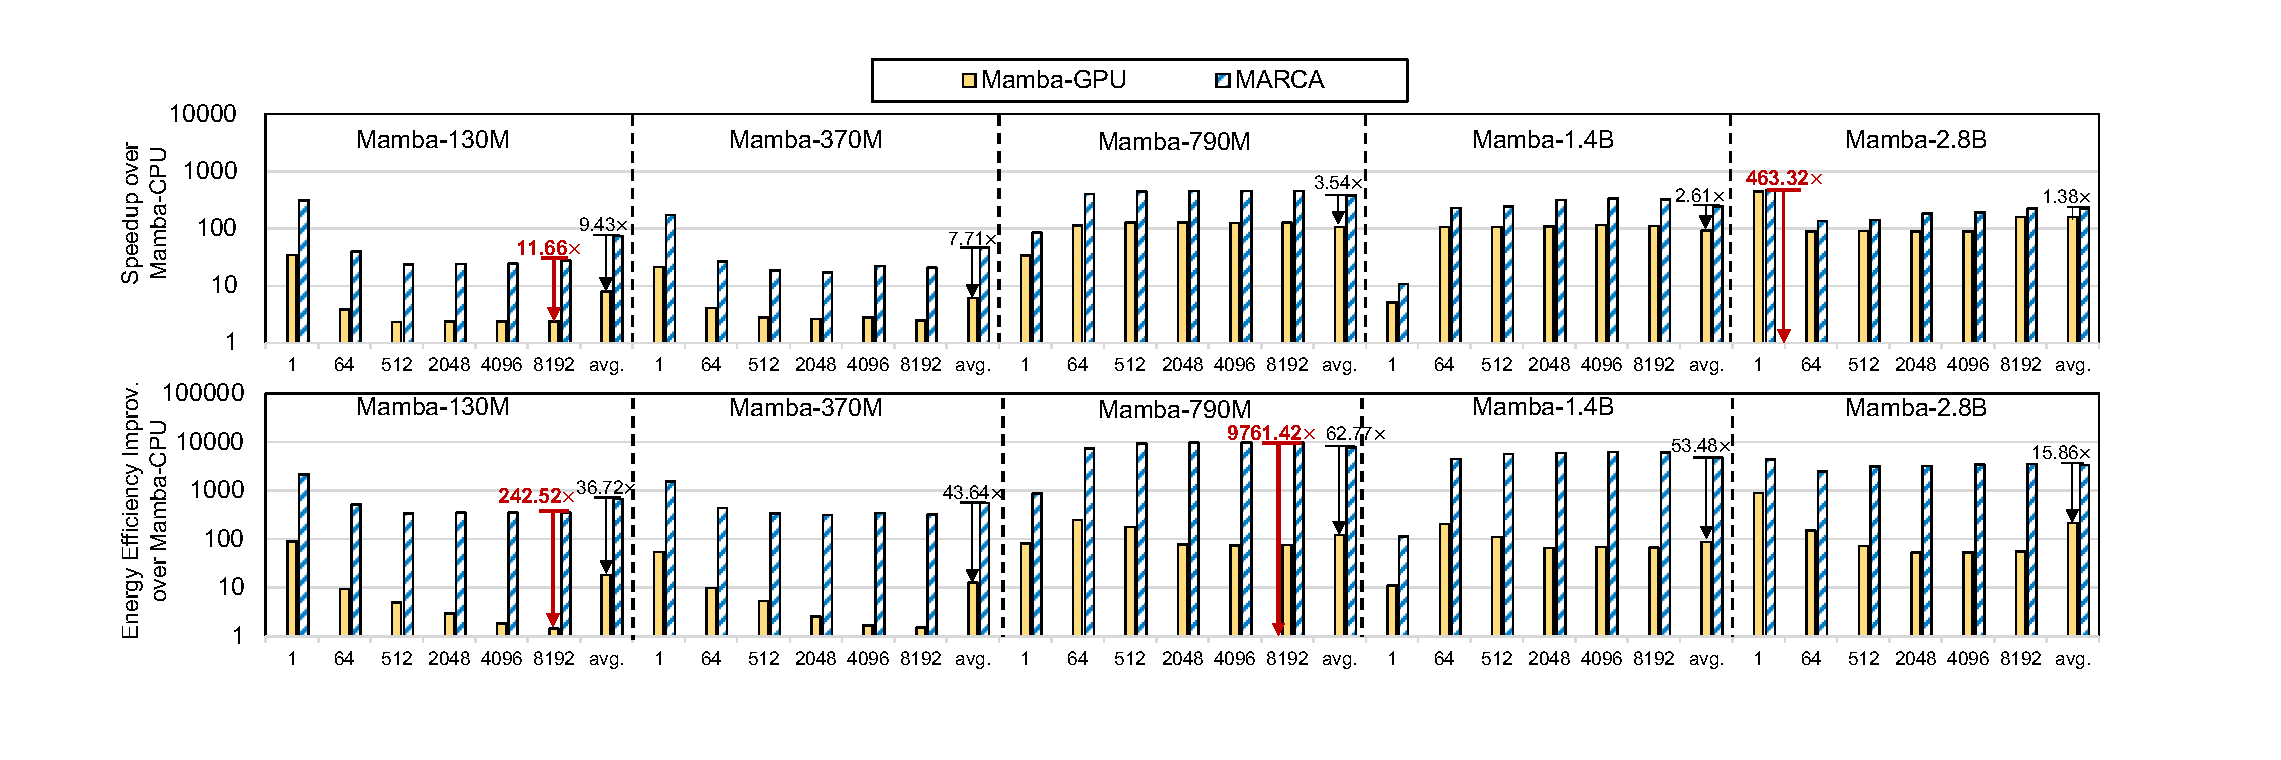
\includegraphics[width=0.99\textwidth]{figures/experiment/speedup.pdf}
%   \vspace{-10pt}
%   \caption{Comparison of speedup and energy efficiency improvement to Mamba-CPU and Mamba-GPU on Mamba models with different input sequence length.}
%   \vspace{-13pt}
%   \label{fig:speedup}
% \end{figure*}

% \subsection{Hardware Evaluations}
% We compare our work with Mamba-CPU and Mamba-GPU in terms of speedup and energy consumption,
% Finally, the area and power of our design is presented.

% % \textbf{\textit{\underline{Speedup.}}}
% \textbf{Speedup.}
% Figure~\ref{fig:speedup} top depicts that \we achieves up to 463.32$\times$/11.66$\times$ speedup and average 194.26$\times$/4.93$\times$ speedup compared with Mamba-CPU and Mamba-GPU, respectively.
% The performance improvement comes from the reconfigurable architecture, and the intra-operation and inter-operation buffer management strategy. 
% First, the reconfigurable computing unit with several reconfigurable processing element arrays accelerate the computations. 
% Second, the intra-operation input data sharing and inter-operation data sharing methods reduce large redundant data between global memory and on-chip memory.
% % Finally, the nonlinear functions are approximated and decomposed into several element-wise operations to reuse the reconfigurable computing units, which improves hardware utilization.



% % \textbf{\textit{\underline{Energy Consumption.}}}
% \textbf{Energy Efficiency.}
% As Figure~\ref{fig:speedup} bottom shows, \we improves up to 9761.42$\times$/242.52$\times$ and average 3415.55$\times$/42.49$\times$ energy efficiency compared to Mamba-CPU and Mamba-GPU, respectively. 
% We consider the energy consumption of all platforms includes the off-chip memory.

% \textbf{Power and Area.}
% The total power and area of \we are only 10.44 $W$ and 221.88 $mm^2$, respectively. 
% For the on-chip buffer, we use eDRAM to reduce both the area and energy consumption. 
% For the computation precision, we use 32-bit fixed point that is enough to maintain the accuracy of Mamba inference. 
% Table~\ref{tab:pwr_and_area} provides area and power breakdown.
% The on-chip buffer consumes most of power (>60\%) and area ($\sim$80\%) to support more memory access and data sharing for element-wise operations.
% The compute engine consume 38.67\% power and 20.57\% area to perform the linear, element-wise, exponential, and SiLU computations.
% The others are small owing to the simple implementations of normalization, and instruction fetching and decoding.

% \begin{table}[htbp]
% \small
%     \centering
%     \vspace{-10pt}
%     \caption{Layout Characteristics of \we}
%     \vspace{-12pt}
%     \begin{tabular}{cccc}
%         \toprule
%         \textbf{Component} & \textbf{Sub-module} & \textbf{Area} ($mm^2$/\%) & \textbf{Power} ($W$/\%) \\
%         \midrule
%         Inst. Processing & - & 0.45/0.20\% & 0.045/0.43\%\\
%         \midrule
%         Norm. Unit & - & 0.06/0.03\% & 0.003/0.03\%\\
%         \midrule
%         \multirow{4}{*}{Compute Engine} & RPEs & 44.87/20.22\% & 3.92/37.55\% \\
%         & Reduction Trees & 0.47/0.21\% & 0.053/0.51\% \\
%         & Control Unit & 0.32/0.14\% & 0.064/0.61\% \\
%         \cmidrule(lr){2-4}
%         & - & 45.66/20.57\% & 4.037/38.67\% \\
%         \midrule
%         On-chip Buffer & - & 175.71/79.19\% & 6.35/60.87\%\\  
%         \midrule
%         Total & - & 221.88/100\% & 10.44/100\%\\ 
%         \bottomrule
%     \end{tabular}
%     \vspace{-12pt}
%     \label{tab:pwr_and_area}
% \end{table}


% \subsection{Ablation Study}
% % We also present an ablation study to validate the superiority of our RCU over the Tensor Core-based architecture and our buffer management strategy over the no sharing (naive) strategy. 

% \textbf{Speedup of RCU over Tensor Core.}
% Figure~\ref{fig:ablation} top left shows the speedup from 1.41$\times$ to 11.95$\times$ over Tensor Core-based architecture with different sequence length in Mamba. 

% \textbf{Normalized area of RPE.}
% In Figure~\ref{fig:ablation} top right, we compare the normalized PE area overhead by supporting different nonlinear functions.
% It shows that our reusable RPE only increases 14\% area overhead.

% \textbf{Normalized memory access improvement.}
% Figure~\ref{fig:ablation} bottom reveals the normalized global memory access with out buffer management strategy. When the sequence is short, linear operations are dominant, the intra-BM reduces 73\% memory access significantly. The inter-BM reduces 49\% memory access with long sequence.

% \begin{figure}[!t]
%   \centering
%   % \vspace{-5pt}
%   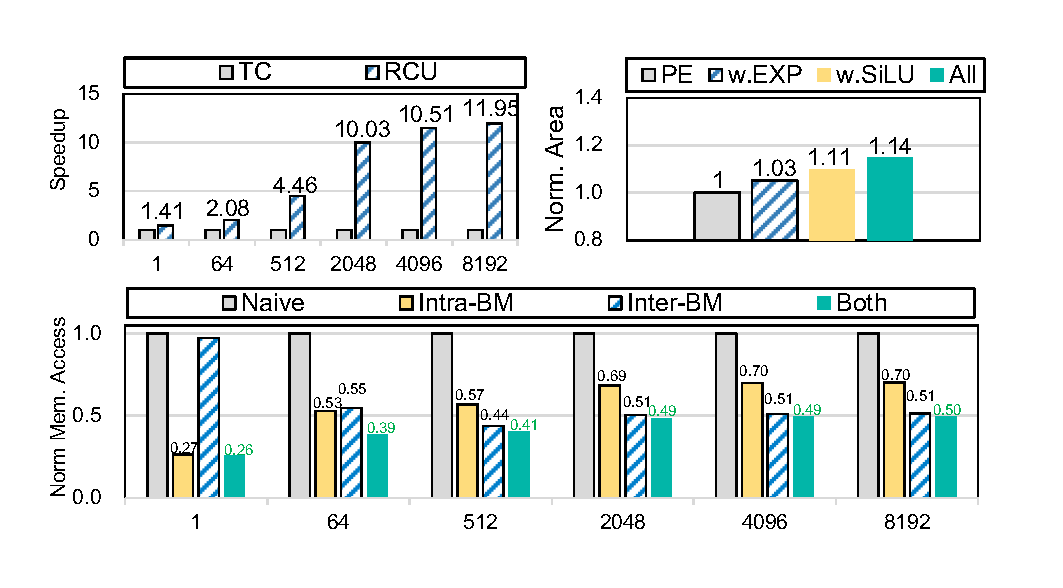
\includegraphics[width=0.47\textwidth]{figures/experiment/ablation.pdf}
%   \vspace{-15pt}
%   \caption{Ablation study: (1) Speedup of RCU over Tensor Core. (2) Normalized area of RPE. (3) Normalized memory access of intra-/inter-operation buffer management strategy.}
%   \vspace{-15pt}
%   \label{fig:ablation}
% \end{figure}

% % \begin{figure}[!t]
% %   \centering
% %   % \vspace{-10pt}
% %   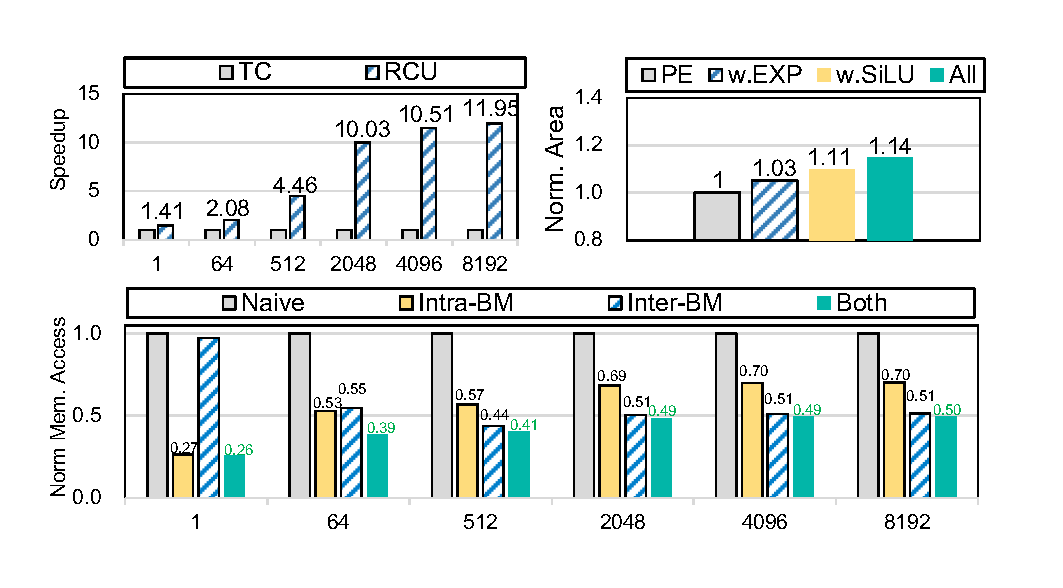
\includegraphics[width=0.48\textwidth]{figures/experiment/ablation.pdf}
% %   \vspace{-20pt}
% %   \caption{Ablation study 2: Normalized memory access of operation-wise buffer management strategy.}
% %   \vspace{-10pt}
% %   \label{fig:ablation2}
% % \end{figure}